\section{The Scattering Transform} \label{sec:ch4:scatternet}
While we have introduced the scattering trasnform before, we clarify the format
we use for this chapter's analysis. 

We use the $\DTCWT$ based scatternet introduced in the previous chapter 
\autoref{alg:ch3:dtcwt_scat} as a front end  with $J=M=2$. Consider a single
channel input signal $x(\xy)$, $\xy \in \reals[2]$.

The zeroth order \textbf{scatter} coefficient is the lowpass output of a $J$
level FB: 
\begin{equation}
  S_0x(\xy) \definedas x(\xy) \conv \phi_J(\xy)
\end{equation}
This is invariant to translations of up to $2^J$ pixels\footnote{From here on,
we drop the $\xy$ notation when indexing $x$, for clarity.}. In exchange for
gaining invariance, the $S_0$ coefficients have lost a lot of information
(contained in the rest of the frequency space). The remaining energy of $x$ is
contained within the first order \textbf{wavelet} coefficients:
\begin{equation}
  W_1x(\xy, j_1, \theta_1) \definedas x \conv \psi_{j_1, \theta_1}
\end{equation}
for $j_1\in\{1, 2\}, \theta_1\in\{1,2, \ldots, 6\}$. We will want to
retain this information in these coefficients to build a useful classifier.

Let us call the set of available scales and orientations $\Lambda_1$ and use
$\lambda_1$ to index it.  For both Morlet and $\DTCWT$ implementations, $\psi$
is complex-valued, i.e., $\psi = \psi^r + j\psi^i$ with $\psi_r$ and $\psi_i$
forming a Hilbert Pair, resulting in an analytic $\psi$.
 This analyticity provides a source of invariance --- small input shifts in $x$
 result in a phase rotation (but little magnitude change) of the complex wavelet
 coefficients\footnote{In comparison to a system with purely real filters such
 as a CNN, which would have rapidly varying coefficients for small input shifts
 \cite{kingsbury_complex_2001}.}.

Taking the magnitude of $W_1$ gives us the first order propagated
signals:
\begin{equation}
  U_1x(\lambda_1, \xy) \definedas |x \conv \psi_{\lambda_1}| 
    = \sqrt{(x \conv \psi^r_{\lambda_1})^2 + (x \conv \psi^i_{\lambda_1})^2}
\end{equation}
The first order scattering coefficient makes $U_1$ invariant up to our
scale $J$ by averaging it:
\begin{equation}
  S_1x(\lambda_1, \xy) \definedas |x \conv \psi_{\lambda_1}| \conv \phi_J
\end{equation}
This has $6\x 2 = 12$ output channels for each input channel. Later in this
chapter we will want to distinguish between the first and second scale
coefficients of the $S_1$ terms, which we will do by moving the $j$ index
to a superscript. I.e., $S_1^1$ and $S_1^2$ refer to the set of 6 $S_1$ terms
at the first and second scales.

Higher order scattering coefficients recover the information lost by
averaging $U_1$, and are defined as:
\begin{eqnarray}
  W_{m} &=& U_{m-1} \conv \psi_{\lambda_{m}} \\
  U_{m} &=& |W_{m}| \\
  S_{m} &=& U_m \conv \phi_J
\end{eqnarray}

Previous work shows that for natural images we get diminishing returns after
$m=2$. The second order scattering coefficients are defined only on paths of
increasing energy\cite{bruna_invariant_2013} as:
\begin{equation}
  S_2x(\lambda_1, \lambda_2, \xy) \definedas ||x \conv \psi_{\lambda_1}|
  \conv \psi_{\lambda_2}| \conv \phi_J
\end{equation}
As we only go on the paths of increasing energy $j_1 = 1$, $j_2=2$. This then
has $6\x6 = 36$ output channels per input channel.

Our output is then a stack of these 3 outputs:
\begin{equation}
  Sx = \{S_0x, S_1x, S_2x\}
\end{equation}
with $1+12+36=49$ channels.

\subsection{Scattering Color Images}\label{sec:ch4:colour}
A wavelet transform like the $\DTCWT$ accepts single channel input, while we
often work on RGB images. This leaves us with a choice. We can either:
\begin{enumerate}
  \item Apply the wavelet transform (and the subsequent scattering operations)
    on each channel independently. This would triple the output size to $3C$.
  \item Define a frequency threshold below which we keep color information, and
    above which, we combine the three channels.
\end{enumerate}
The second option uses the well known fact that the human eye is far less sensitive 
to higher spatial frequencies in color channels than in luminance channels. 
This also fits in with the first layer filters seen in the well known
Convolutional Neural Network, AlexNet. Roughly one half of the filters were low
frequency color `blobs', while the other half were higher frequency, grayscale,
oriented wavelets. 

For this reason, we choose the second option for the
architecture described in this chapter. We keep the 3 color
channels in our $S_0$ coefficients, but work only on grayscale for high orders 
(the $S_0$ coefficients are the lowpass bands of a J-scale wavelet transform, so
we have effectively chosen a color cut-off frequency of $2^{-J} \frac{f_s}{2}$).

We combine the three channels by modifying our magnitude operation from \eqref{eq:ch3:magbias} 
to now be:
\begin{equation}\label{eq:ch4:colour_mag}
 r_s = \sqrt{x_r^2 + y_r^2 + x_g^2 + y_g^2 + x_b^2 + y_b^2 + b^2} - b
\end{equation}
Where $x_r, x_g, x_b$ are the real parts of the wavelet response for the red,
green and blue channels, and $y$ is the corresponding imaginary part. This only
affects the $S_1$ coefficients, and the $S_2$ coefficients then are calculated
as normal. 

An alternative to \eqref{eq:ch4:colour_mag} is to simply combine the colours
before scattering into a luminance channel. However we choose to use \eqref{eq:ch4:colour_mag}
instead as this has the ability to detect colour edges with constant luminance.

The resulting scattering output now has $3 + 12 + 36 = 51$ channels at $1/16$ the
spatial input size.

\section{The Inverse Scatter Network}\label{sec:ch4:descatternet}
\begin{figure}[t]
  \centering
  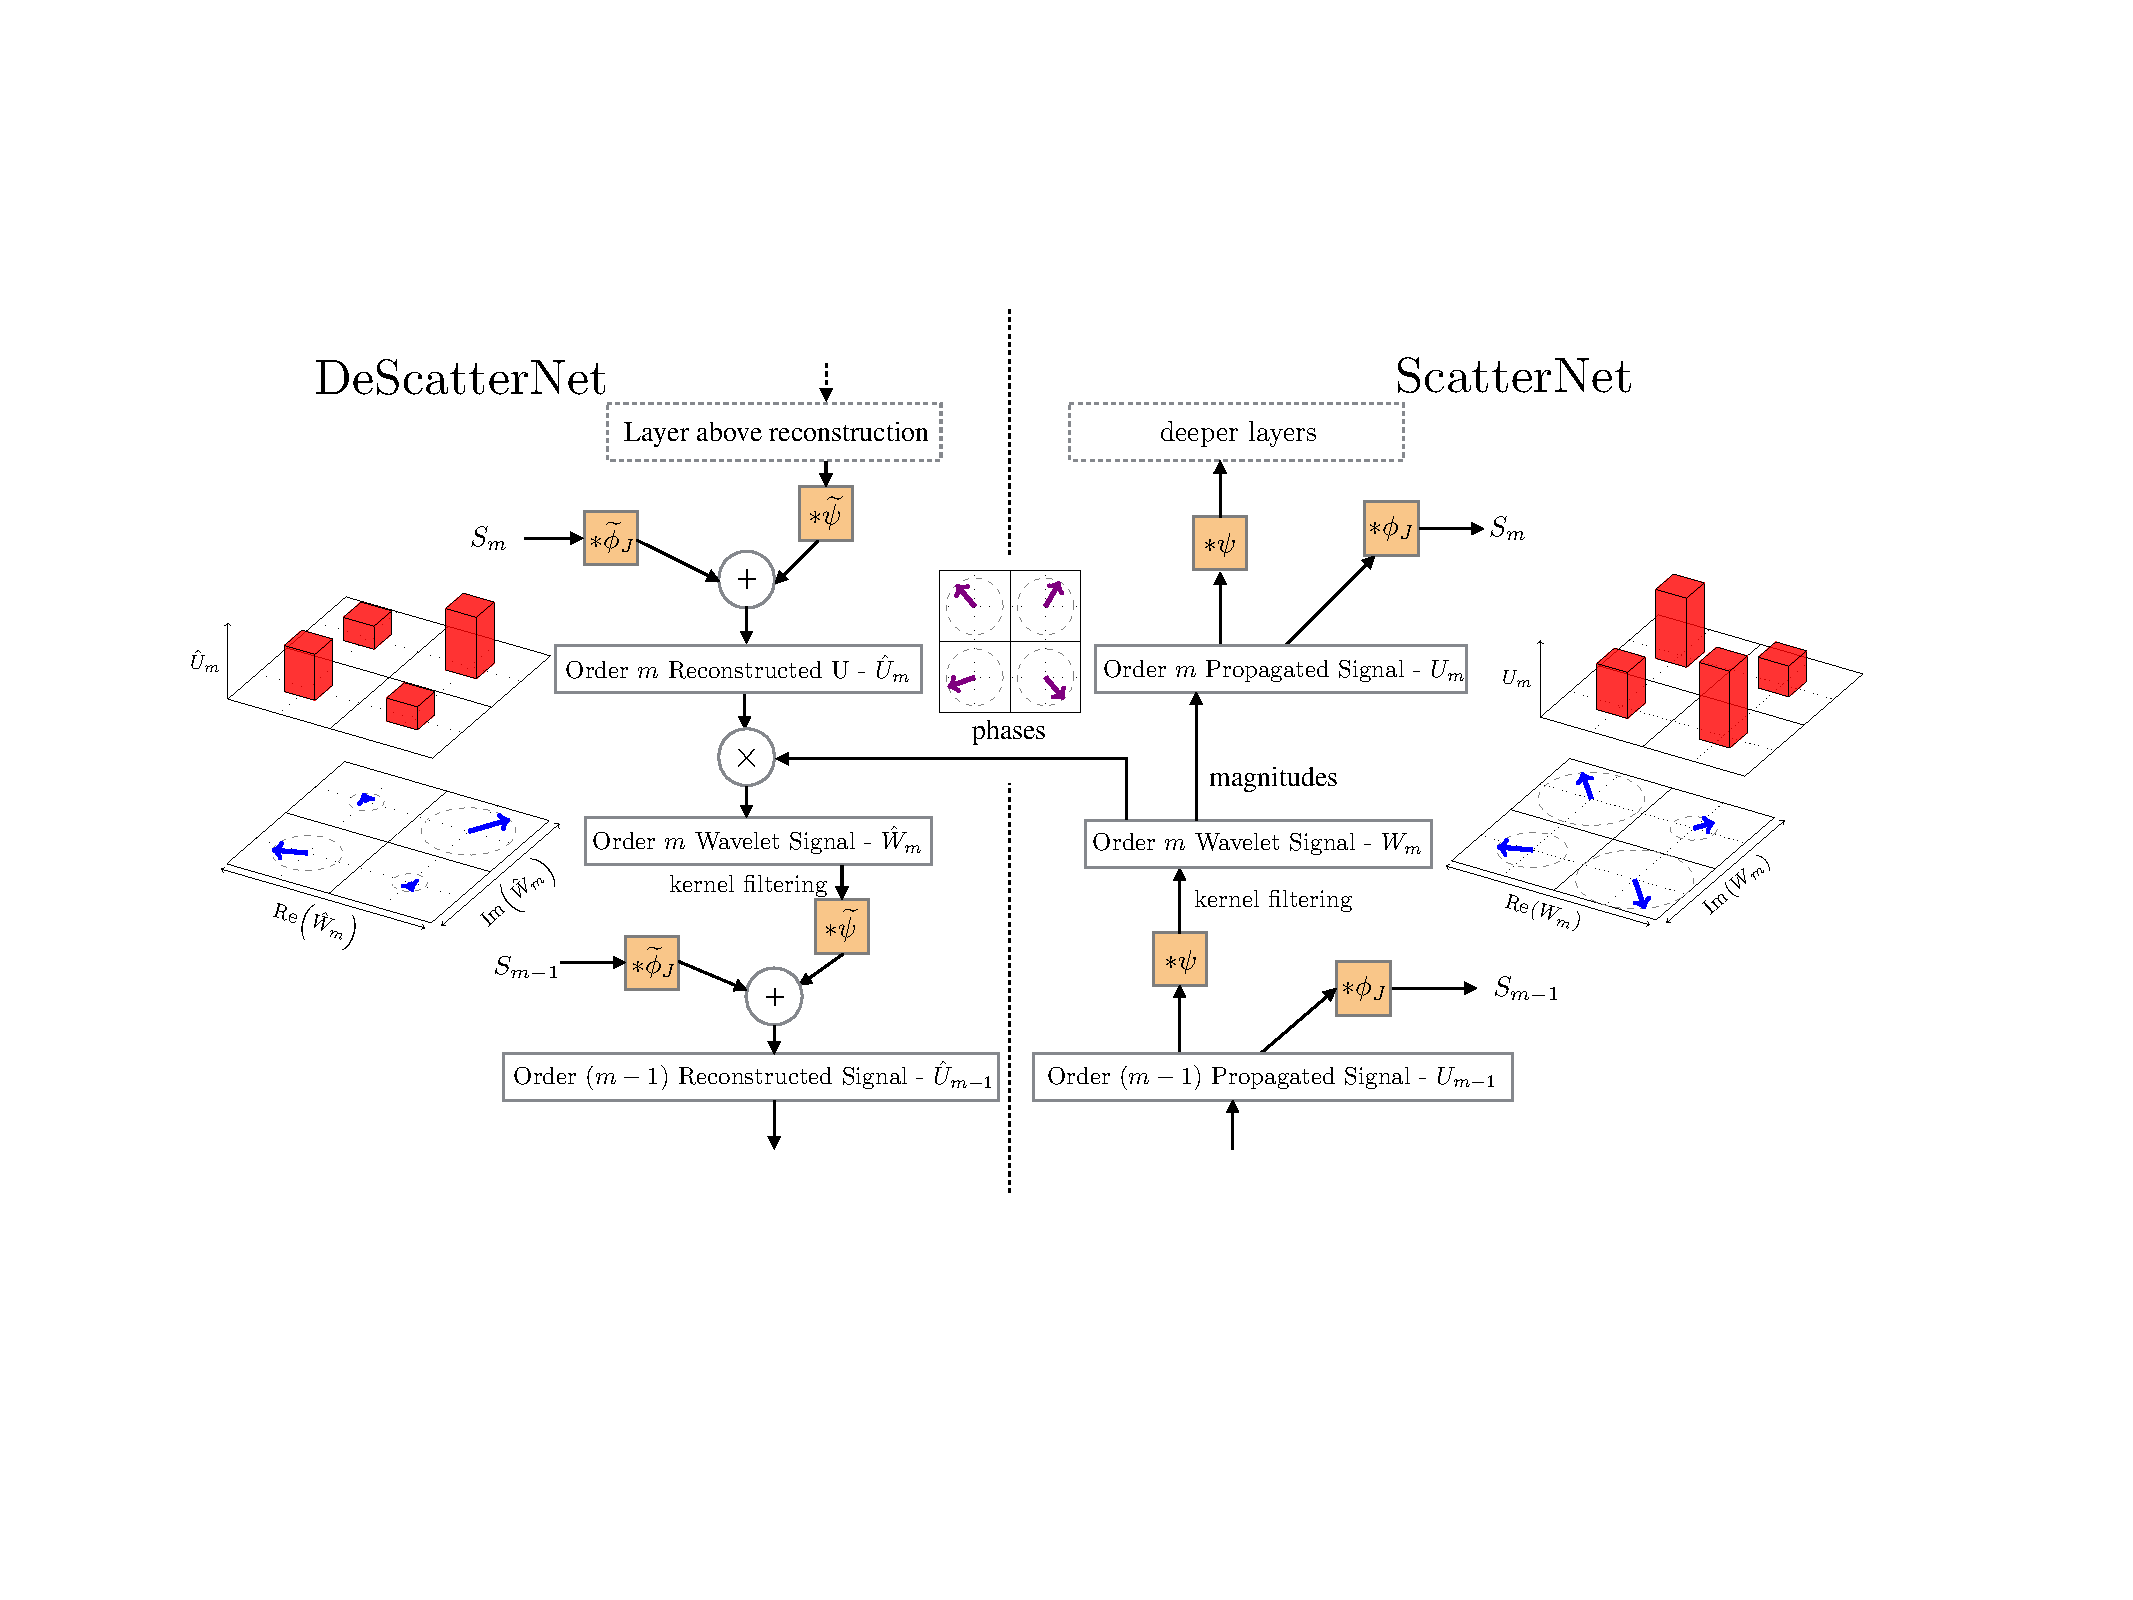
\includegraphics[width=\textwidth, trim={3cm 7cm 4cm 6cm},clip]{\imgpath/descat.pdf}
  \mycaption{The Descattering Network}{Comprised of a DeScattering layer (left)
  attached to a Scattering layer (right).  We are using the same convention as
  \cite{zeiler_visualizing_2014} Figure 1 - i.e. the input signal starts in the
  bottom right hand corner, passes forwards through the ScatterNet (up the right
  half), and then is reconstructed in the DeScatterNet (downwards on the left
  half).  The DeScattering layer will reconstruct an approximate version of the
  previous order's propagated signal. The $2\x 2$ grids shown around the image
  are either Argand diagrams representing the magnitude and phase of small
  regions of \emph{complex} (De)ScatterNet coefficients, or bar charts showing
  the magnitude of the \emph{real} (De)ScatterNet coefficients (after applying
  the modulus non-linearity). For reconstruction, we need to save the discarded
  phase information and reintroduce it by multiplying it with the reconstructed
  magnitudes.}
  \label{fig:ch4:descat}
\end{figure}

We now introduce our inverse scattering network. This allows us to back project
scattering coefficients to the image plane; it is inspired by the
DeconvNet used by Zeiler and Fergus in
\cite{zeiler_visualizing_2014} to look into the deeper layers of CNNs. Like
the DeConvNet, the inverse Scattering Network is similar to backpropping a
single strong activation (rather than usual gradient terms). 

We emphasize that instead of thinking about perfectly reconstructing $x$ from
$S\in \reals[C\x H'\x W']$, we want to see what signal/pattern in the input image caused
a large activation in each channel. This gives us a good idea of what each
output channel is sensitive to, or what it extracts from the input. 
Note that we do not use any of the log normalization layers described in
\cite{oyallon_deep_2015, singh_dual-tree_2017}.

\subsection{Inverting the Low-Pass Filtering}
Going from the $U$ coefficients to the $S$ coefficients involved convolving by
a low pass filter, $\phi_J$ followed by decimation to make the output $(H\x
2^{-J})\x (W\x2^{-J})$.  $\phi_J$ is a purely real filter, and we can `invert'
this operation by interpolating $S$ to the same spatial size as $U$ and convolving with
the mirror image of $\phi_J$, $\widetilde{\phi}_J$ (this is equivalent to the
transpose convolution described in \cite{zeiler_visualizing_2014}). 
\begin{equation}
  \label{eq:ch4:s_hat}
  \hat{S}_{m} = S_{m} \conv \widetilde{\phi}_J
\end{equation}
This will not recover $U$ as it was on the forward pass, but will recover all
the information in $U$ that caused a strong response in $S$.

\subsection{Inverting the Magnitude Operation}
In the same vein as \cite{zeiler_visualizing_2014}, we face a difficult
task in inverting the non-linearity in our system. 
% It has been proven that for
% particular wavelets, we can recover the phase from their modulus
% \cite{waldspurger_phase_2012}, but this is not a trivial operation. Instead, we
We lend inspiration from the switches introduced in the DeconvNet; the
switches in a DeconvNet save the location of maximal activations so that
on the backwards pass activation layers could be unpooled trivially. We do an
equivalent operation by saving the phase of the complex activations. On the
backwards pass we reinsert the phase to give our recovered $W$. 
\begin{equation}
  \label{eq:ch4:w_hat}
  \hat{W}_{m} = \hat{U}_{m}e^{j\theta_{m}}
\end{equation}

\subsection{Inverting the Wavelet Decomposition}
Using the $\DTCWT$ makes inverting the wavelet transform simple, as we
can simply feed the coefficients through the synthesis filter banks to regenerate
the signal. For complex $\psi$, this is convolving with the conjugate transpose
$\widetilde{\psi}$: 

\begin{eqnarray}
  \label{eq:ch4:x_hat}
  \hat{U}_{m-1} &=& \hat{S}_{m-1} + \hat{W}_{m} \\
              &=& S_{m-1} \conv \widetilde{\phi}_J + \sum_{j, \theta} W_{m}(\bm{u}, j,
  \theta) \conv \widetilde{\psi}_{j, \theta}
\end{eqnarray}

\begin{figure}[tp]
  \centering
  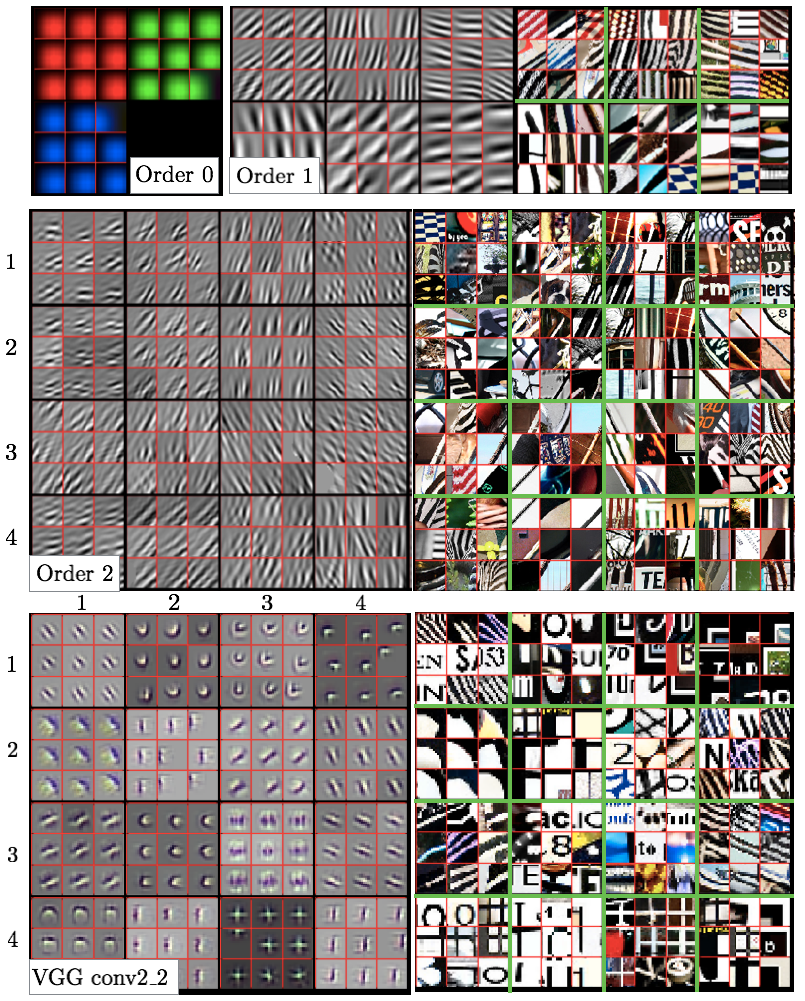
\includegraphics[width=0.9\textwidth]{\imgpath/deconv_images.png}
  \caption{Visualization of a random subset of features from $S_0$ (all
  3), $S_1$ (6 from the 12) and $S_2$ (16 from the 36) scattering
    outputs. We record the top 9 activations for the chosen features and project
    them back to the pixel space. We show them alongside the input image patches
    which caused the large activations. We also include reconstructions from
    layer conv2\_2 of VGG Net \cite{simonyan_very_2014}(a popular CNN, often used
    for feature extraction) for reference --- here we display 16 of the 128
    channels. The VGG reconstructions were made with a CNN DeconvNet based on
    \cite{zeiler_visualizing_2014}. Image best viewed digitally.}
  \label{fig:ch4:reconstructions}
\end{figure}

\section{Visualization with Inverse Scattering}
\label{sec:ch4:visualization}

To examine our ScatterNet, we scatter all of the images from ImageNet's validation
set and record the top 9 images which most highly activate each of the $C$
channels in the ScatterNet. This is the \emph{identification} phase (in which no
inverse scattering is performed). 

Then, in the \emph{reconstruction}
phase, we load in the $9\x C$ images, and scatter them one by one. We take the
resulting 52 channel output vector and mask all but a single value in the
channel we are currently examining.

This 1-sparse tensor is then presented to the inverse scattering network from
\autoref{fig:ch4:descat} and projected back to the image space. Some results of this
are shown in \autoref{fig:ch4:reconstructions}. This figure shows reconstructed
features from the layers of a ScatterNet. For a given output channel, we show
the top 9 activations projected independently to pixel space. For the first and
second order coefficients, we also show the patch of pixels in the input image
which cause this large output. We display activations from various scales
(increasing from first row to last row), and random orientations in these
scales. 

The order 1 scattering (labelled with `Order 1' in
\autoref{fig:ch4:reconstructions}) coefficients look quite similar to the first
layer filters from the well known AlexNet CNN \cite{krizhevsky_imagenet_2012}.
This is not too surprising, as the first order scattering coefficients are
simply a wavelet transform followed by average pooling. They are responding to
images with strong edges aligned with the wavelet orientation. 

The second order coefficients (labelled with `Order
2' in \autoref{fig:ch4:reconstructions}) appear very similar to the order
1 coefficients at first glance.
They too are sensitive to edge-like features, and some of them (e.g.\ third row,
third column and fourth row, second column) are mostly just that. These are
features that have the same oriented wavelet applied at both the first and
second order.  Others, such as the nine in the top left square (first row, first column), 
and top right square (first row, fourth column) are more sensitive to
checker-board like patterns. Indeed, these are activations where the orientation
of the wavelet for the first and second order scattering were far from each
other ($15\degs$ and $105\degs$ for the first row, first column and $105\degs$
and $45\degs$ for the first row, fourth column).

For comparison, we include reconstructions from the second layer of the
well-known VGG CNN\@ (labelled with `VGG conv2\_2', in
\autoref{fig:ch4:reconstructions}). These were made with a DeconvNet, following the
same method as \cite{zeiler_visualizing_2014}. Note that while some of
the features are edge-like, we also see higher order shapes like corners,
crosses and curves.

These reconstructions show that the features extracted from ScatterNets vary
significantly from those learned in CNNs after the first order. In many
respects, the features extracted from a CNN like VGGNet look preferable for use
as part of a classification system.

% \subsection{Hybrid ScatterNet Visualization}
% Visualize some of the features of a convnet.

\section{Channel Saliency}
To get another heuristic on the importance of the ScatterNet channels, let us examine
the effect on inference scores observed when zeroing out Scattering channels.
\cite{zeiler_visualizing_2014, zhou_object_2014} have done similar studies but
over patches of the input image, with the former using a patch of grey values as
the occlusion mask, and the latter using a set of random pixels. 

We must be careful to occlude with a sensible mask, the $S_0x$, $S_1x$ and $S_2x$
all have very different probability densities. Assuming $x~\mathcal{N}(0, \sigma^2I)$ 
(already a fairly weak assumption),
the pdf of $S_0x$ will also be a zero mean gaussian. However, the distributions
of $S_1x$ and $S_2x$ are more complex - the real and imaginary parts of the
$\DTCWT$ are sparse, with a Laplacian distribution a commonly used estimate for each,
however they are strongly correlated. Choosing a sensible random mask is
therefore difficult, so we instead use a constant mask. Analysis of the
datasets show that zero is very close to the maximum likelihood value for each
channel so we occlude channels by simply setting them to zero at every spatial
location.

\subsection{Experiment Setup}
We take a network similar to the one from
\autoref{tab:ch3:scat_arch} but using the colour operation described in 
\autoref{sec:ch4:colour} so the scattering output has 51 output channels. We further
set $C=50$ so the conv1 layer has 100 channels. We train this network
on the same 3 datasets - CIFAR-10, CIFAR-100 and Tiny ImageNet, and report the
drop in classification scores on the validation set after removing one channel at
a time. 

We additionally display the weight matrix for the first learned layer of the
network trained on Tiny ImageNet. This gives us a second perspective on the
channel importance by looking at the relative weights of the ScatterNet channels
passed on to the successive 100 channels. The weight matrix is convolutional
filter of size $w \in \reals[100\x 51\x 3\x 3]$. We define:
\begin{equation}
  A^{rms}_{c, f} &=& \sqrt{\frac{\sum_{i,j} w[f, c, i, j]^2}{{\sum_f \sum_{i,j} w[f, c, i, j]^2}}}
\end{equation}
This gives us a matrix $A^{rms}$ (for root mean squared) which has columns of
unit energy representing the different output channels after conv1. The row
values then show how much each scattering channel contributes to each output
channel. This is shown in \autoref{}.

\subsection{Discussion}
First we look at Tiny ImageNet in \autoref{fig:ch4:occlusion1}.
Note that when any of the $S_0$ channels are removed, 
the validation accuracy drops sharply for all 3 datasets. A similar result
happens when any of the $S_1$ channels are zeroed out. 

For both the first and second scales of the first order coefficients, 
$S_1^1$ and $S_1^2$, there are two channels that seem less
important - the second and fifth channels, corresponding to the $45\degs$ and
$135\degs$ wavelets. Often the high-high portion of the first scale coefficients
are considered mostly noise \cite{}, but this does not explain why the $45\degs$
and $135\degs$ channels for the second scale coefficients are also less
important. A possible interesting conclusion to be drawn from this is that the
dataset does not have as many diagonal edges in it as horizontal and vertical
edges. 

To test this, we retrain the network but this time rotate the input
images randomly $30\degs$ clockwise or anti-clockwise in both training and
validation. We then rerun the occlusion experiment for all channels and plot the
resulting changes in \autoref{fig:ch4:ti_rotated_occlusion}. Interestingly, for
this network, the $45\degs$ and $135\degs$ wavelets for $S_1^2$ are now the most
important of the 6, which validates our assumption. The corresponding wavelets
for $S_1^1$ have become more important, but it is likely that they remain less
salient because of the effects of the higher bandwidth for the diagonal
wavelets.

Comparatively, the $S_2$ channels have little effect on the classification score
when individually masked. Interestingly, the four largest drops in accuracy for
$S_2$ happen when $\theta_1 = \theta_2 = 15\degs, 75\degs, 105\degs, 165\degs$.
When $\theta_1 \neq \theta_2$ we saw the ripple like patterns in
\autoref{fig:ch4:visualizations}, and we see here that the network has mostly
learned to not depend on them.



\begin{figure}
  \vspace{-2cm}
  \centering
  \subfloat[Tiny ImageNet]{\vspace{-1cm}
    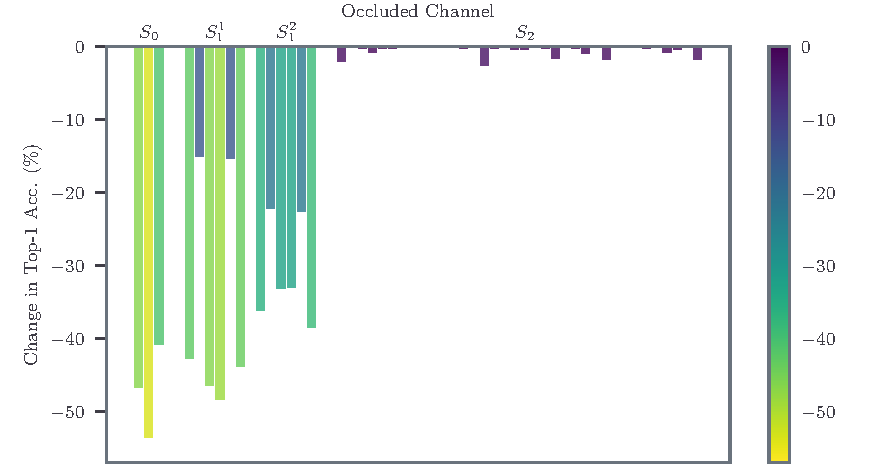
\includegraphics[width=15cm,height=8cm]{\imgpath/ti_occlusion_colour.pdf}
    \label{fig:ch4:ti_occlusion}
    }
    \\
  \subfloat[Rotated Tiny ImageNet]{
    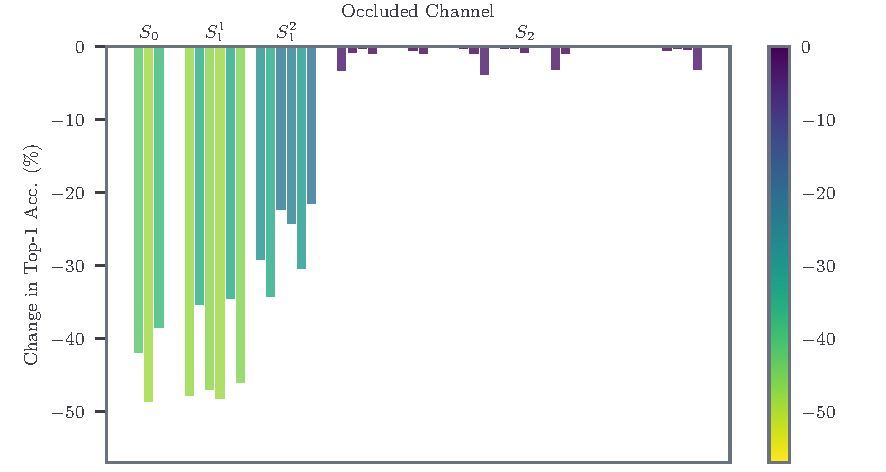
\includegraphics[width=15cm,height=8cm]{\imgpath/ti_rotated_occlusion_colour.pdf}
    \label{fig:ch4:ti_rotated_occlusion}
    }\vspace{-0.3cm}
  \mycaption{Tiny ImageNet changes in accuracy from channel occlusion}{Numbers
  reported are the drop in final classification accuracy when a channel is set
  to zero. The bars are coloured relative to their magnitude to aid seeing the
  differences for the $S_1$ coefficients. \subref{fig:ch4:ti_occlusion} When 
  any of the lowpass channels $S_0$ are removed, the classification accuracy
  drops sharply, note that the middle channel, corresponding to green, is
  unsurprisingly the most important of the three colours. The first scale, first
  order scattering coefficients $S_1^1$ are slightly more important than the
  second scale coefficients. Interestingly, the second and fifth orientations
  for both of these are comparatively less important orientations. These
  correspond to the $45\degs$ and $135\degs$ wavelets. The 36 $S_2$ coefficients
  have very little individual effect on the}
  \label{fig:ch4:occlusion1}
\end{figure}
take a trained hybrid network, l
take the ScatterNet built in the previous chapter \autoref{tab:ch3:scat_arch}, and
iterate through the output channels , turning them off one by one and measuring the effect this
has on classification score. 

We do this for the ScatterNet 


\section{Corners, Crosses and Curves}
\label{sec:ch4:corners}

\begin{figure}[t]
  \centering
  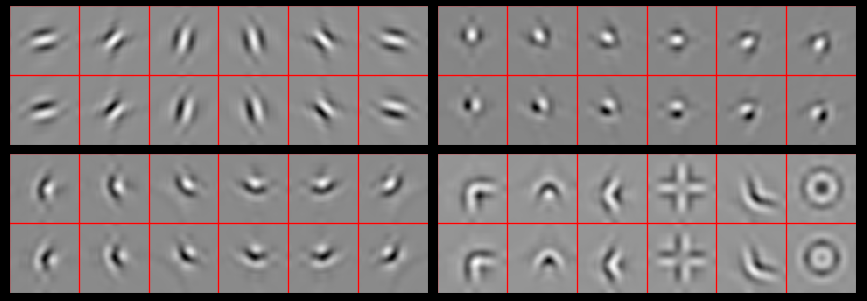
\includegraphics[width=0.9\textwidth]{\imgpath/figure3.png}
  \mycaption{Shapes possible by filtering across the wavelet orientations with
  complex coefficients}{All shapes are shown
  in pairs: the top image is reconstructed from a purely real output, and the
  bottom image from a purely imaginary output. These `real' and `imaginary' shapes 
  are nearly orthogonal in the pixel space (normalized dot product $<0.01$ for
  all but the doughnut shape in the bottom right, which has $0.15$) but produce
  the same $U'$, something that would not be possible without the complex
  filters of a ScatterNet.  Top left - reconstructions from $U_1$ (i.e.\ no
  cross-orientation filtering). Top right- reconstructions from $U_1'$ using
  a $1\x 1\x 12$ Morlet Wavelet, similar to what was done in the `Roto-Translation'
  ScatterNet described in \cite{sifre_rotation_2013, oyallon_deep_2015}. Bottom
  left - reconstructions from $U_1'$ made with a more general $1\x 1\x 12$
  filter, described in \autoref{eq:ch4:simple_corner}. Bottom
  right - some reconstructions possible by filtering a general $3\x 3\x 12$ filter.}
  \label{fig:ch4:newshapes}
\end{figure}


We build on these two systems, showing that with carefully designed complex
filters applied across the complex spatial coefficients of a 2-D $\DTCWT$,  
we can build filters that are sensitive to more recognizable shapes like
those commonly seen in CNNs, such as corners and curves (\autoref{sec:ch4:corners}). 
% The work in \cite{oyallon_deep_2015} demonstrated that second order scattering
% coefficients are necessary, and give a large increase in accuracy over using
% just the first order coefficients.
% We now propose an additional layer that can be added to our
% ScatterNet with ease, which generates filters sensitive to these higher order
% shapes. In fact, we have a great deal of flexibility with what shapes we can be
% sensitive to.

\cite{sifre_rotation_2013} and \cite{oyallon_deep_2015} introduced the idea of
a `Roto-Translation' ScatterNet. Invariance to rotation could be made by
applying averaging (and bandpass) filters across the $L$ orientations 
from the wavelet transform \emph{before} applying the complex modulus.
Momentarily ignoring the form of the filters they apply, referring to them
as $F_k\in \complexes[L]$, we can think of this stage as stacking the $L$
outputs of a complex wavelet transform on top of each other, and convolving
these filters $F_k$ over all spatial locations of the wavelet coefficients $W_m
x$ (this is equivalent to how filters in a CNN are fully connected
in depth):
\begin{equation}
  V_m x(\bm{u}, j, k) = W_{m}x \conv F_k = \sum_{\theta} W_{m}x(\bm{u}, j, \theta)
F_k(\theta)
\end{equation}
We then take the modulus of these complex outputs to make a second propagated
signal:
\begin{equation}
  U_{m}'x \definedas |V_{m}x| = |W_{m}x \conv F_k| = |U_{m-1}x
  \conv \psi_{\lambda_{m}} \conv F_k|
\end{equation}
We present a variation on this idea, by filtering with a more general 
$F\in \complexes[H\x W\x 12]$. We use $F$ of length 12 rather than 6, as we use
the $L=6$ orientations and their complex conjugates; each wavelet is a 30$\degs$
rotation of the previous, so with 12 rotations, we can cover the full
$360\degs$. 
% The filters can be shared across scales J to produce the same shapes at
% different scales. Further, if $F\in \complexes[1\x 1\x 12]$, then we can 
% create 12 orientations of the same shape by simply rotating the
% filter coefficients in $F$ by one sample along the third dimension; each sample
% shift rotating the shape by $30\degs$. For more general shaped $F$, we can still
% trivially get rotations of the shape, but it requires rotating the coefficients
% spatially too.

\autoref{fig:ch4:newshapes} shows some reconstructions from these $V$ coefficients.
Each of the four quadrants show reconstructions from a different class of
ScatterNet layer. 
All shapes are shown in real and imaginary Hilbert-like pairs; the top images in
each quadrant are reconstructed from a purely real $V$, while the bottom inputs
are reconstructed from a purely imaginary $V$. This shows one level of invariance of
these filters, as after taking the complex magnitude, both the top and the
bottom shape will activate the filter with the same strength. In comparison, for
the purely real filters of a CNN, the top shape would cause a large output, and
the bottom shape would cause near 0 activity (they are nearly orthogonal to each
other).

In the top left, we display the 6 wavelet filters for reference (these were
reconstructed from $U_1$, not $V_1$). In the top right of the figure we see some
of the shapes made by using the $F$'s from the Roto-Translation ScatterNet
\cite{sifre_rotation_2013, oyallon_deep_2015}.  The bottom left is where we
present some of our novel kernels. These are simple corner-like shapes made 
by filtering with ${F\in \complexes[1\x 1\x 12]}$
% \vspace{-10pt}
\begin{equation} \label{eq:ch4:simple_corner}
  F = [1, j, j, 1, 0, 0, 0, 0, 0, 0, 0, 0]
\end{equation}
The six orientations are made by rolling the coefficients in $F$ along one
sample (i.e. $[0, 1, j, j, 1, 0,\ldots]$, $[0,0,1,j,j,1,0,\ldots]$,
$[0,0,0,1,j,j,1,0, \ldots]$ \ldots). Coefficients roll back around (like
circular convolution) when they reach the end.

Finally, in the bottom right we see shapes made by 
${F \in \complexes[3\x 3\x 12]}$. Note that with the exception of the 
ring-like shape which has 12 non-zero coefficients, all of these shapes were
reconstructed with $F$'s that have 4 to 8 non-zero coefficients of a possible 
64. These shapes are now beginning to more closely resemble the more complex
shapes seen in the middle stages of CNNs. 

\section{Discussion}
This paper presents a way to investigate what the higher orders of a ScatterNet
are responding to - the DeScatterNet described in \autoref{sec:ch4:descatternet}.
Using this, we have shown that the second `layer' of a ScatterNet 
responds strongly to patterns that are very dissimilar to those that highly activate the
second layer of a CNN\@. As well as being dissimilar to CNNs, visual inspection of the
ScatterNet's patterns reveal that they may be less useful for discriminative
tasks, and we believe this may be causing the current gaps in state-of-the-art
performance between the two. 

We have presented an architectural change to ScatterNets that can make it
sensitive to more recognizable shapes. We believe that using this new layer is
how we can start to close the gap, making more generic and descriptive
ScatterNets while keeping control of their desirable properties. 

% \pagebreak
% References should be produced using the bibtex program from suitable
% BiBTeX files (here: strings, refs, manuals). The IEEEbib.bst bibliography
% style file from IEEE produces unsorted bibliography list.
% -------------------------------------------------------------------------
